We will now construct a learning algorithm that can find a set of coefficients for the partitions of the preconditioner such that the preconditioned system have a decreased solver iteration count. Then we will test the algorithm on the four matrices from the previous section. The reason we construct a leaning algorithm and not using an already established Machine Learning algorithm is the need to define a loss function. The standard loss functions expect a continues input, if then we use the solver iteration count as the input to those functions it might run into unexpected behavior. And because the condition number is only a bound for the error it is not the ideal measure of improvement.

The approach we take to learning the coefficients of the preconditioner takes inspiration from stochastic gradient decent. Starting with randomly generated initial coefficients for the partitions with a predetermined number of partitions. Then choose one of the coefficient at random to be change by value generated from some distribution. With this new changed preconditioner the new system is solved to get a solver iteration count to use as a measure, to determine of the change made to the coefficient had a positive or negative effect on the solver iteration. If it decreases the change is kept, otherwise if it increases the iteration count it is rejected. Regardless of the outcome a new coefficient is chosen to be changed. This procedure is then repeated for a number of predetermined learning steps. Pseudocode for this procedure can be seen in Algorithm \ref{alg: initial learn}.

The new parameters that needs to be determined for the learning algorithm is: number of learning steps and how to change the partition coefficients. To choose which coefficient that will be changed we have decided on uniform distribution for which coefficient to be changed, with the knowledge that for larger number of partitions, a larger number of learning steps is needed to explore each coefficient thoroughly. For the value of the change to the coefficient we will use a uniform distribution with mean of zero and different range for each of the four test matrices. Lastly for the number of learning steps we set this to 300 for all test matrices. The number of partitions and the distribution parameters can be seen in table \ref{table: initial learn param}.

\begin{algorithm}
    \caption{Preconditioner learning algorithm}\label{alg: initial learn}
    \begin{algorithmic}
        % \Require $n \geq 0$
        \Require Matrix \(A\) and vector \(b\) form \(Ax=b\)
        \State \(M^{-1} \gets \) Generate initial preconditioner
        \State \(k \gets\) Solver iteration count for \(M^{-1}Ax=M^{-1}b\)
        \Loop{ \(i=1,2,\ldots\)}
            \State \(M^{-1}_{new} \gets \) Changed \(M^{-1}\)
            \State \(k_{new} \gets\) Solver iteration count for \(M^{-1}_{new}Ax=M^{-1}_{new}b\)
            \If{ \(k_{new} < k\)}
                \State \(k \gets k_{new}\)
                \State \(M^{-1} \gets M^{-1}_{new}\)
            \EndIf
        \EndLoop
    \end{algorithmic}
\end{algorithm}


\begin{table}[H]
    \center
    \begin{tabular}{|l|r|r|r|r|}
        \hline
        Matrix &\begin{tabular}{@{}l@{}}Number of\\ partitions\end{tabular}&\begin{tabular}{@{}l@{}}Coefficient\\ distribution\end{tabular} & \begin{tabular}{@{}l@{}}Change\\ distribution\end{tabular}  \\ \hline
        eris1176 & 8 & \(N(0,0.1^2)\) & \(Uni(-0.5,0.5)\)\\
        fidap004 & 8 & \(N(0,0.05^2)\) & \(Uni(-0.1,0.1)\)\\
        orsirr\_1 & 15 & \(N(0.01^2)\) & \(Uni(-1,1)\)\\
        sherman5 & 4 & \(N(0,0.05^2)\) & \(Uni(-0.01,0.01)\)\\\hline
    \end{tabular}
    \caption{The learn parameters for the different matrices with each column corresponding to in order the name of the matrix; number of partitions in the preconditioner; the distribution for the initial partition coefficient; the distribution for the changing the values of the coefficients.}
    \label{table: initial learn param}
\end{table}



\begin{figure}[H]
    \center
    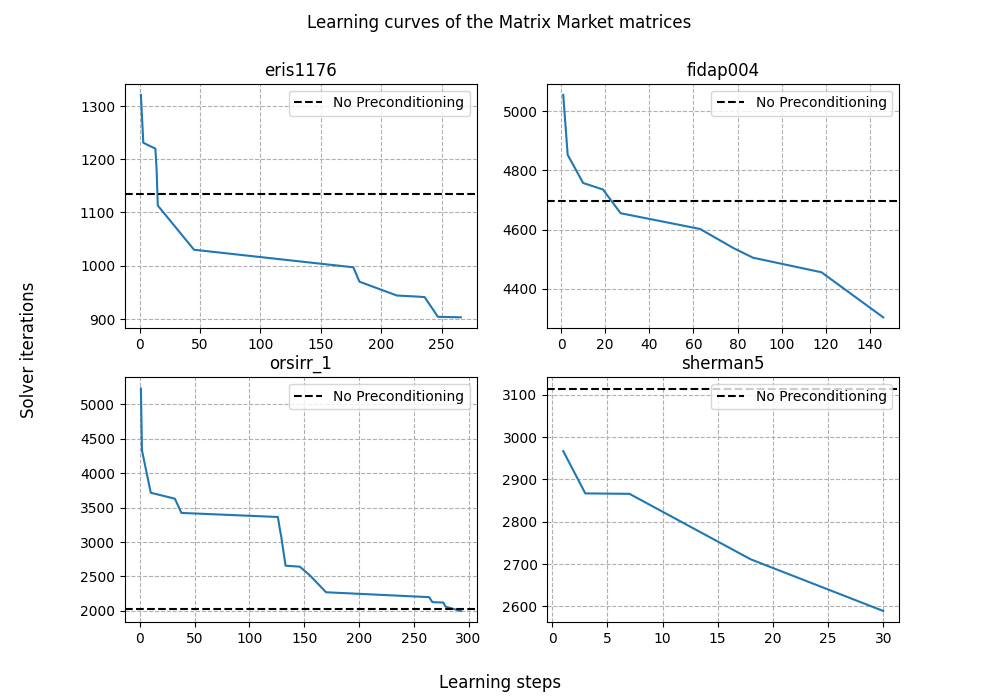
\includegraphics[width=0.8\textwidth]{plots/initial_learn.png}
    \caption{Learning curves of each of the four test matrices. Where the blue line shows the solver iteration count, with data point for each learning step the algorithm accepted a new preconditioner, and a dashed line indicating the unpreconditioned solver iteration count for corresponding matrix.}
    \label{fig: initial learn}
\end{figure}
\newpage
What immediately can be seen from the learning curves in figure \ref{fig: initial learn}, is that our algorithm does what we set out to do.  Because it finds a better set of coefficient that form a better preconditioner and that it uses fewer solver iterations than the corresponding system with a preconditioner applied. The final solver iteration counts can be seen in table \ref{table: initial learn stat}. Another thing, that is not immediately obvious, is that very few of the learning steps a new preconditioner got accepted, at most 17 out the 300 iterations for orsirr\_1 but this may be because of the initial preconditioner making the system much worse and therefore easier to learn. It is difficult to tell if this is a real problem because of the fact the all learned preconditioner works better than with no preconditioner applied, even when the initial preconditioner makes the solver iteration count much larger. The few number of improvements for sherman5 could be contributed to the fact that the initial preconditioner already improves the system and starts at a lower solver iteration count than the unpreconditioned, so it may have learned what it can with few steps. This difficult to say from sherman5's data, but it is clear from the runs for the three other matrices that this learning method can work.

\begin{table}[H]
    \center
    \begin{tabular}{|l|c|c|c|c|}
        \hline
        Matrix & Final & Compare v Non & \begin{tabular}{@{}l@{}}Learning\\ improvement\end{tabular} & \begin{tabular}{@{}l@{}}Number of \\ improvements\end{tabular}\\ \hline
        eris1176 & 903 & 231 & 418 & 14\\
        fidap004 & 4304 & 391 & 750 & 10 \\
        orsirr\_1 & 1998 & 27& 3233 & 17 \\
        sherman5 & 2589 & 526 & 378 & 5 \\\hline
    \end{tabular}
    \caption{Table of data from the learning of the preconditioner with row for each for the matrices and columns corresponding to in order the name of the matrix; the solver iteration count for the final preconditioner; how many fewer solve iterations the preconditioned used compared to the unpreconditioned system; solver iteration count difference between the initial preconditioned system and the final preconditioned system; the number of times a a change to the preconditioned was accepted.}
    \label{table: initial learn stat}
\end{table}